\documentclass[usletter]{article}
\usepackage{graphicx}
\usepackage{amsfonts}
\usepackage{amsthm}
\usepackage{amsmath}
\usepackage{amssymb}
\usepackage{scribe}
\usepackage[margin=1.5in]{geometry}

\usepackage{xcolor}
\usepackage{xfrac}
\usepackage{tikz}
\usetikzlibrary{chains,fit,shapes}
\newcommand*\circled[1]{\tikz[baseline=(char.base)]{
            \node[shape=circle,draw,inner sep=2pt] (char) {#1};}}

\begin{document}


\makeheader{Nakul Khambhati}                              % your name
           {January 18, 2023}                          % lecture date
           {3}                                       % lecture number
           {Time Bounds and Robustness}  % lecture title

\noindent
In the previous lecture, we completed a proof that demonstrates that
constant depth circuits cannot compute parity. We also reviewed Turing Machines (TMs) and defined them formally.
Finally, we discussed an \(O(n)\) algorithm for computing \verb|PALINDROME|. 

In this lecture, we will explore efficiency by defining time bounded TMs. We argue that TMs are robust to most minor modifications. 
However, replacing a \(k\)-tape TM with a single tape TM results in a quadratic slowdown for some languages.
Finally, we revisit \verb|PALINDROME| and introduce crossing sequences to exhibit a lower bound on the slowdown caused by this restriction. 

\section{Efficiency}
We will now narrow our focus to TMs that efficiently solve problems.
Before we can define efficiency, we need to introduce some notation. Consider a function \(f: \left\{ 0,1 \right\}^* \to \left\{  0,1 \right\}^*\). 
Intuitively, this function \(f\) is solving some problem where the input and output are both expressed in binary. Technically, however, this can be any
arbitrary mapping of binary strings. Also, let \(T: \mathbb{N} \to \mathbb{N}\) be a natural-valued function. This function represents the time-bound that we impose
upon our Turing Machine. 

\begin{definition}
    A TM \(M\) computes a function \(f\) in time \(T(n)\) if when started with arbitrary input \(x \in \left\{ 0,1 \right\}^*\), \(M\) halts within \(T(|x|)\) steps with \(f(x)\) 
    written on the output tape. Here, \(|x|\) denotes the bit-length of \(x\).
\end{definition}

\begin{example}
    The TM \(M\) that we constructed last lecture to solve \verb|PALINDROME| runs in time \(O(n)\). Here, and several times later, \(n\) is used as a placeholder for \(|x|\).
\end{example}

Let's restrict our attention to functions that output \(0\) or \(1\) instead of arbitrarily long strings. These functions are called languages or decision problems.

\begin{definition}
    A language is a subset \(L \subset \left\{ 0,1 \right\}^*\). \(M\) decides a language \(L\) if \(M\) computes the associated characteristic function \(f_L(x): \left\{ 0,1 \right\}^* \to \left\{ 0,1 \right\}\).
    \begin{equation}
        f_L(x) = 
        \left\{
            \begin{array}{lr}
                1, & \text{if } x \in L\\
                0, & \text{otherwise}
            \end{array}
        \right\}
    \end{equation}
\end{definition}

This equips us with the tools necessary to introduce certain classes of languages.

\begin{definition}
    \(\mathbf{DTIME}(T(n))\) is the family of all languages \(L\) that are decidable within time \(cT(n)\) for some constant \(c > 0\). 
\end{definition}

\begin{definition}
    The class \(\mathbf{P} = \bigcup\limits_{k = 1}^{\infty}\mathbf{DTIME}(n^k)\) contains all languages \(L\) that can be solved by some TM \(M\) running in polynomial time. 
    These are considered to be the languages that can be solved \textit{efficiently}.
\end{definition}

\begin{remark}
    Note that while the class \(\mathbf{DTIME}(T(n))\) is defined in terms of TMs, 
the objects being classified are languages and not TMs.
\end{remark}

It is worth discussing the appearance of the constant \(c\) in Definition 3.4.
According to this definition, a language \(L\), which is decidable by \(M\) that runs in \(100n\), lies in the same class as a language \(L'\) 
that some \(M'\) decides in \(0.01n\). Is this because constant factors don't matter in complexity theory? Or is there a deeper reason? As it turns out, 
both are true. For starters, the exact specifications of a machine may increase the runtime of an algorithm by a constant factor. However, the same algorithm 
run on different types of classical\footnote[1]{Quantum computers can increase the speed of certain algorithms by more than constant factor but these have not yet been physically realized.} 
machines will belong to the same class \(\mathbf{DTIME}(T(n))\). At a deeper level, the linear speedup theorem \cite{textbook} states that given any real \(c > 0\) and any \(k\)-tape Turing machine solving a problem
in time \(T(n)\), there is another \(k\)-tape machine that solves the same problem in time at most \(T(n)/c + 2n + 3\), where \(k > 1\). This brings us to our next topic of discussion \(-\) the robustness of Turing Machines. 
 
\section{Robustness of TMs}
As it turns out, our model of a TM is robust in the sense that the theory is largely unaffected by minor modifications. Since most of the details in our definition of a TM are arbitrary,
we want a model that doesn't change significantly with these parameters. Some variations we can make to our TM are restricting its alphabet to the bare minimum, allowing the tape to be infinitely long in both directions,
and insisting that our TM uses a single tape.

\begin{itemize}
\item[1.] \textbf{Restricting the alphabet}: In our definition of a TM, we allow the alphabet
\(\Gamma\) to be arbitrarily long. However, we can restrict ourselves to the alphabet 
\(\Gamma = \left\{ 0,1, \triangleright, \square \right\}\) and increase the running time
by only a constant factor. 

\begin{theorem}
    If \(f: \left\{ 0,1 \right\}^*\) is computable in time \(T(n)\) with alphabet \(\Gamma\), then \(f\) is computable in time \(O(T(n)\log \Gamma) = O(T(n))\) with alphabet \(\left\{ 0,1,\triangleright, \square \right\}\).
\end{theorem}

Matan provides the intuition here by explaining that we can 
create a mapping from the original alphabet to the set \(\left\{ 0,1 \right\}^*\). 
\begin{figure}[h]
\centering
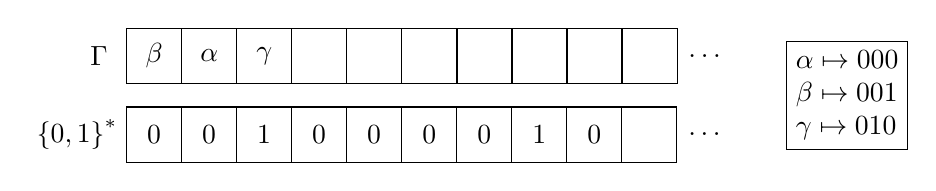
\begin{tikzpicture}
% \tikzstyle{every path}=[very thick]

\edef\sizetape{0.7cm}
\tikzstyle{tmtape}=[draw,minimum size=\sizetape]
% \tikzstyle{tmhead}=[arrow box,draw,minimum size=.5cm,arrow box
% arrows={east:.25cm, west:0.25cm}]

%% Draw TM tape
\begin{scope}[shift={(-0.5cm,0cm)},start chain=1 going right,node distance=-0.15mm]
    \node [on chain=1,tmtape,draw=none] {\(\Gamma\)};
    \node [on chain=1,tmtape] {\(\beta\)};
    \node [on chain=1,tmtape] {\(\alpha\)};
    \node [on chain=1,tmtape] {\(\gamma\)};
    \node [on chain=1,tmtape] {};
    \node [on chain=1,tmtape] {};
    \node [on chain=1,tmtape] {};
    \node [on chain=1,tmtape] {};
    \node [on chain=1,tmtape] {};
    \node [on chain=1,tmtape] {};
    \node [on chain=1,tmtape] {};
    \node [on chain=1,tmtape,draw=none] {$\ldots$};
    % \node [on chain=1] {\textbf{Input/Output Tape}};
\end{scope}
\begin{scope}[shift={(-0.78cm,-1cm)}, start chain=1 going right,node distance=-0.15mm]
    \node [on chain=1,tmtape,draw=none] {\(\left\{ 0,1 \right\}^*\)};
    \node [on chain=1,tmtape] {\(0\)};
    \node [on chain=1,tmtape] {\(0\)};
    \node [on chain=1,tmtape] {\(1\)};
    \node [on chain=1,tmtape] {\(0\)};
    \node [on chain=1,tmtape] {\(0\)};
    \node [on chain=1,tmtape] {\(0\)};
    \node [on chain=1,tmtape] {\(0\)};
    \node [on chain=1,tmtape] {\(1\)};
    \node [on chain=1,tmtape] {\(0\)};
    \node [on chain=1,tmtape] {};
    \node [on chain=1,tmtape,draw=none] {$\ldots$};
    % \node [on chain=1] {\textbf{Input/Output Tape}};
\end{scope}
    
\node[draw,align=left] at (9,-0.5) {\(\alpha \mapsto 000\)\\ \(\beta \mapsto 001\)\\ \(\gamma \mapsto 010\)};


\end{tikzpicture}
\caption{Translating from \(\Gamma\) to \(\left\{ 0,1 \right\}^*\)}
\end{figure}

Then, we replace every instance of a symbol from the original alphabet with its corresponding
binary representation and provide the TM with instructions to interpret it accordingly. 
Assuming that our original alphabet \(\Gamma\) had length \(|\Gamma|\), we need \(\log \Gamma\)
bits to uniquely identify each symbol. Therefore, this results in a constant (with respect to 
input length \(n\)) increase in the running time. Note that there will be some other constant factors involved in this slowdown as well. For example, 
the modified TM will need additional states to store the symbols being read. 

\item[2.] \textbf{Bidirectional tape}: By definition, we allow the TM to extend infinitely to the right. We can instead allow it to extend infinitely in both directions. In practice, this is very useful while solving certain problems. Surprisingly, though, this does not 
make the TM any more powerful. 
\begin{theorem}
    If \(f: \left\{  0,1 \right\}^* \to \left\{ 0,1 \right\}^*\) is computable in time \(T(n)\) with bidirectional tapes, then \(f\) is computable in time \(O(T(n))\) using standard tapes. 
\end{theorem}

\begin{proof}
    Assume that \(f\) is computable by a bidirectional TM \(M\). Let's denote \(M\)'s alphabet as \(\Gamma\). 
    We will construct a TM \(\tilde{M}\) with alphabet \(\Gamma^2\). Now, in each cell, \(\tilde{M}\) can represent a pair \((\sigma, \tau)\) of symbols in \(\Gamma\). We construct \(\tilde{M}\) by \textit{folding} \(M\)'s tapes \cite{arorabarak} at some point from left to right. This reduces the tapes from bidirectional to standard.
    
    \begin{figure}[h]
    \centering
    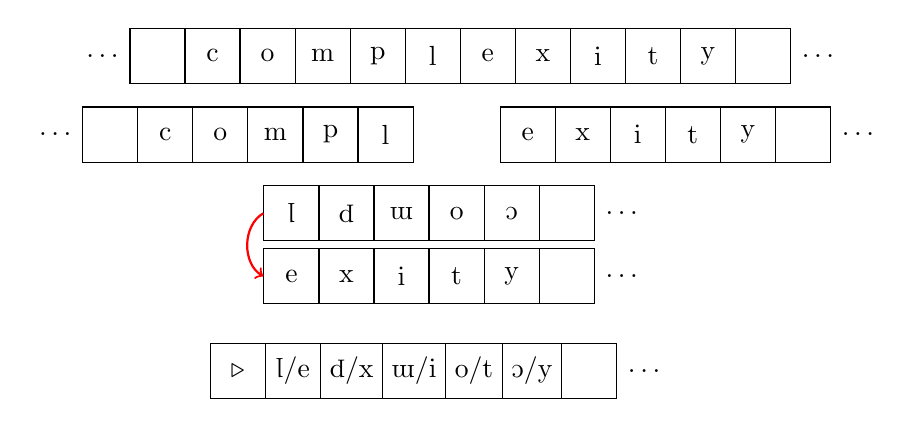
\begin{tikzpicture}
        % \tikzstyle{every path}=[very thick]
        
        \edef\sizetape{0.7cm}
        \tikzstyle{tmtape}=[draw,minimum size=\sizetape]
        % \tikzstyle{tmhead}=[arrow box,draw,minimum size=.5cm,arrow box
        % arrows={east:.25cm, west:0.25cm}]
        
        %% Draw TM tape
        \begin{scope}[shift={(1.6cm,0cm)},start chain=1 going right,node distance=-0.15mm]

            \node [on chain=1,tmtape,draw=none] {\(\ldots\)};
            \node [on chain=1,tmtape] {};
            \node [on chain=1,tmtape] {c};
            \node [on chain=1,tmtape] {o};
            \node [on chain=1,tmtape] {m};
            \node [on chain=1,tmtape] {p};
            \node [on chain=1,tmtape] {l};
            \node [on chain=1,tmtape] {e};
            \node [on chain=1,tmtape] {x};
            \node [on chain=1,tmtape] {i};
            \node [on chain=1,tmtape] {t};
            \node [on chain=1,tmtape] {y};
            \node [on chain=1,tmtape] {};
            \node [on chain=1,tmtape,draw=none] {$\ldots$};
            % \node [on chain=1] {\textbf{Input/Output Tape}};
        \end{scope}

        \begin{scope}[shift={(1cm,-1cm)},start chain=1 going right,node distance=-0.15mm]
            \node [on chain=1,tmtape,draw=none] {\(\ldots\)};
            \node [on chain=1,tmtape] {};
            \node [on chain=1,tmtape] {c};
            \node [on chain=1,tmtape] {o};
            \node [on chain=1,tmtape] {m};
            \node [on chain=1,tmtape] {p};
            \node [on chain=1,tmtape] {l};

            % \node [on chain=1,tmtape,draw=none] {$\ldots$};
            % \node [on chain=1] {\textbf{Input/Output Tape}};
        \end{scope}

        \begin{scope}[shift={(7cm,-1cm)},start chain=1 going right,node distance=-0.15mm]
            % \node [on chain=1,tmtape,draw=none] {\(\ldots\)};
            \node [on chain=1,tmtape] {e};
            \node [on chain=1,tmtape] {x};
            \node [on chain=1,tmtape] {i};
            \node [on chain=1,tmtape] {t};
            \node [on chain=1,tmtape] {y};
            \node [on chain=1,tmtape] {};

            \node [on chain=1,tmtape,draw=none] {$\ldots$};
            % \node [on chain=1] {\textbf{Input/Output Tape}};
        \end{scope}


        \begin{scope}[shift={(4cm,-2cm)},start chain=1 going right,node distance=-0.15mm]
            % \node [on chain=1,tmtape,draw=none] {\(\ldots\)};
            % \node [on chain=1,tmtape] {};
            \node [on chain=1,tmtape] (a) {\raisebox{\depth}{\scalebox{-1}[-1]{l}}};
            \node [on chain=1,tmtape] {\raisebox{\depth}{\scalebox{-1}[-1]{p}}};
            \node [on chain=1,tmtape] {\raisebox{\depth}{\scalebox{-1}[-1]{m}}};
            \node [on chain=1,tmtape] {\raisebox{\depth}{\scalebox{-1}[-1]{o}}};
            \node [on chain=1,tmtape] {\raisebox{\depth}{\scalebox{-1}[-1]{c}}};
            \node [on chain=1,tmtape] {};
            
            \node [on chain=1,tmtape,draw=none] {$\ldots$};
            % \node [on chain=1] {\textbf{Input/Output Tape}};
        \end{scope}

        \begin{scope}[shift={(4cm,-2.8cm)},start chain=1 going right,node distance=-0.15mm]
            % \node [on chain=1,tmtape,draw=none] {\(\ldots\)};
            % \node [on chain=1,tmtape] {};
            \node [on chain=1,tmtape] (b) {e};
            \node [on chain=1,tmtape] {x};
            \node [on chain=1,tmtape] {i};
            \node [on chain=1,tmtape] {t};
            \node [on chain=1,tmtape] {y};
            \node [on chain=1,tmtape] {};

            \node [on chain=1,tmtape,draw=none] {$\ldots$};
            % \node [on chain=1] {\textbf{Input/Output Tape}};

        \end{scope}

        \draw [->,red, thick] (a.west) to [out=210,in=150] (b.west);

        \begin{scope}[shift={(3.32cm,-4cm)},start chain=1 going right,node distance=-0.15mm]
            % \node [on chain=1,tmtape,draw=none] {\(\ldots\)};
            % \node [on chain=1,tmtape] {};

            \node [on chain=1,tmtape] {\(\triangleright\)};
            \node [on chain=1,tmtape] (a) {\raisebox{\depth}{\scalebox{-1}[-1]{l}}/e};
            \node [on chain=1,tmtape] {\raisebox{\depth}{\scalebox{-1}[-1]{p}}/x};
            \node [on chain=1,tmtape] {\raisebox{\depth}{\scalebox{-1}[-1]{m}}/i};
            \node [on chain=1,tmtape] {\raisebox{\depth}{\scalebox{-1}[-1]{o}}/t};
            \node [on chain=1,tmtape] {\raisebox{\depth}{\scalebox{-1}[-1]{c}}/y};
            \node [on chain=1,tmtape] {};
            
            \node [on chain=1,tmtape,draw=none] {$\ldots$};
            % \node [on chain=1] {\textbf{Input/Output Tape}};
        \end{scope}

        % \begin{scope}[shift={(-0.78cm,-1cm)}, start chain=1 going right,node distance=-0.15mm]
        %     \node [on chain=1,tmtape,draw=none] {\(\left\{ 0,1 \right\}^*\)};
        %     \node [on chain=1,tmtape] {\(0\)};
        %     \node [on chain=1,tmtape] {\(0\)};
        %     \node [on chain=1,tmtape] {\(1\)};
        %     \node [on chain=1,tmtape] {\(0\)};
        %     \node [on chain=1,tmtape] {\(0\)};
        %     \node [on chain=1,tmtape] {\(0\)};
        %     \node [on chain=1,tmtape] {\(0\)};
        %     \node [on chain=1,tmtape] {\(1\)};
        %     \node [on chain=1,tmtape] {\(0\)};
        %     \node [on chain=1,tmtape] {};
        %     \node [on chain=1,tmtape,draw=none] {$\ldots$};
        %     % \node [on chain=1] {\textbf{Input/Output Tape}};
        % \end{scope}
        
        
    \end{tikzpicture}
    \caption{Reducing a bidirectional tape to a standard tape}
    \end{figure}

    Now every cell holds two values: its original value before the fold and the symbol in the cell with which it overlaps after the fold. \(\tilde{M}\) also has an additional state for each tape, called FLIP which takes on two values. As the head moves across the tape, this state instructs it to only read one of these symbols (say the first one). This corresponds to the head moving to the right
    in the original TM \(M\). When any of \(M\)'s heads crosses over to the left of its starting position, \(\tilde{M}\) changes its state and starts reading the second symbol instead. In this way, changing the state FLIP corresponds to one of \(M\)'s heads moving across the edge of the fold in the original tape.
    The additional states and extended alphabet only produce a constant increase in runtime. 
\end{proof}

\begin{remark}
    A corollary of this theorem is that we can determine whether a certain language \(L\) is in \(\mathbf{DTIME}(T(n))\) by constructing a bidirectional tape to solve the problem in \(T(n)\). Then, by the theorem, the language is computable in \(O(T(n))\) with standard tapes.
\end{remark}



\item[3.] \textbf{Single tape}: Now we consider the case where we allow our TM \(M\) to have only one tape. This means that
\(M\) uses the same tape to read input, perform intermediate calculations and write output. This case is particularly interesting
because this restriction results in a quadratic slowdown. 

\begin{theorem}
    If \(f: \left\{ 0,1 \right\}^* \to \left\{  0,1 \right\}^*\) is computable in
    time \(T(n)\) on a \(k\)-tape TM then \(f\) is computable in 
    time \(O(T(n)^2)\) on a single tape TM.
\end{theorem}
\begin{proof}
    Let \(M\) be a \(k\)-tape TM that computes \(f\) in time \(T(n)\). As illustrated, 
    it starts with \(k\) tapes and \(k\) heads. At every computational step the heads 
    scan the \(k\) cells directly underneath and use that information, along with the 
    \(M\)'s states, to decide which symbols to write in the cells and which direction 
    to move in afterwards. This parallelism (for \(k \geq 2\)) comes in very handy. 
    For example, in \verb|PALINDROME|, two heads move simultaneously, working together
    to test equality between the \(i^{th}\) and \((n-i)^{th}\) symbols. We wish to simulate
    this behaviour with only \(1\) tape. 

    One simple approach here, which proves to be optimal, is to use a richer alphabet 
    \(\tilde{\Gamma} = (\Gamma \times \left\{ 0,1 \right\})^k\) in \(\tilde{M}\) to keep track
    of the position of the \(k\) heads of \(M\). This way, there is a dedicated extended alphabet
    \(\tilde{\Gamma}_i\) for the \(i^{th}\) tape. Also, each \(\tilde{\Gamma}_i\) is twice as
    large as the original \(\Gamma\) to allow us to mark the location of that tape's head. 
    For this purpose, think of each \(\tilde{\Gamma}_i\) as two copies of \(\Gamma\) \(-\) one with regular symbols \(\sigma\)
    and one with circled symbols \textcircled{\(\sigma\)}. A circled symbol will indicate that in \(M\) a tape's head is above that cell. 
    Now, as illustrated below, we can pretend like \(\tilde{M}\) has one giant head that simultaneously scans through
    all \(k\) tapes together from left to right till it reaches the last symbol.
    
    \begin{figure}[h]
    \centering
    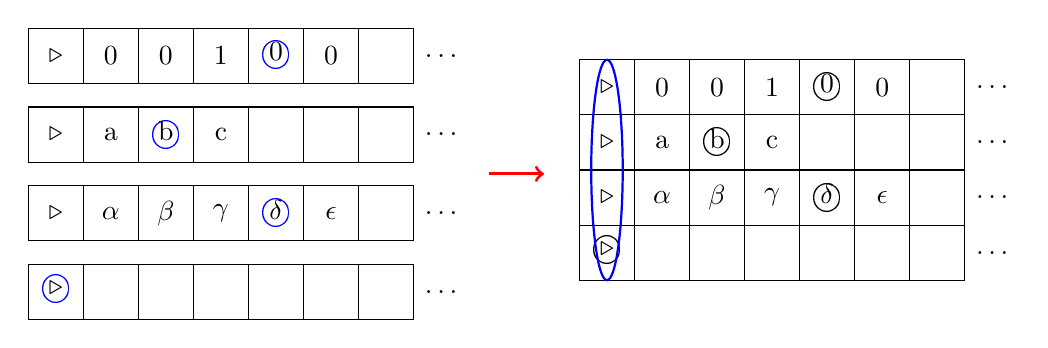
\begin{tikzpicture}
        % \tikzstyle{every path}=[very thick]
        
        \edef\sizetape{0.7cm}
        \tikzstyle{tmtape}=[draw,minimum size=\sizetape]
        % \tikzstyle{tmhead}=[arrow box,draw,minimum size=.5cm,arrow box
        % arrows={east:.25cm, west:0.25cm}]
        
        %% Draw TM tape
        \begin{scope}[shift={(0cm,0cm)},start chain=1 going right,node distance=-0.15mm]
            \node [on chain=1,tmtape] {\(\triangleright\)};
            \node [on chain=1,tmtape] {\(0\)};
            \node [on chain=1,tmtape] {\(0\)};
            \node [on chain=1,tmtape] {\(1\)};
            \node [on chain=1,tmtape] {\(\textcolor{blue}{\textcircled{\textcolor{black}{0}}}\)};
            \node [on chain=1,tmtape] {\(0\)};
            \node [on chain=1,tmtape] {};
            % \node [on chain=1,tmtape] {};

            \node [on chain=1,tmtape,draw=none] {$\ldots$};
            % \node [on chain=1] {\textbf{Input/Output Tape}};
        \end{scope}
        \begin{scope}[shift={(0cm,-1cm)},start chain=1 going right,node distance=-0.15mm]
            \node [on chain=1,tmtape] {\(\triangleright\)};
            \node [on chain=1,tmtape] {a};
            \node [on chain=1,tmtape] {\(\textcolor{blue}{\textcircled{\textcolor{black}{b}}}\)};
            \node [on chain=1,tmtape] {c};
            \node [on chain=1,tmtape] {};
            \node [on chain=1,tmtape] {};
            \node [on chain=1,tmtape] {};
            % \node [on chain=1,tmtape] {};
            \node [on chain=1,tmtape,draw=none] {$\ldots$};
            % \node [on chain=1] {\textbf{Input/Output Tape}};
        \end{scope}
        \begin{scope}[shift={(0cm,-2cm)},start chain=1 going right,node distance=-0.15mm]
            \node [on chain=1,tmtape] {\(\triangleright\)};
            \node [on chain=1,tmtape] {\(\alpha\)};
            \node [on chain=1,tmtape] {\(\beta\)};
            \node [on chain=1,tmtape] {\(\gamma\)};
            \node [on chain=1,tmtape] {\(\textcolor{blue}{\textcircled{\textcolor{black}{\(\delta\)}}}\)};
            \node [on chain=1,tmtape] {\(\epsilon\)};
            \node [on chain=1,tmtape] {};
            % \node [on chain=1,tmtape] {};

            \node [on chain=1,tmtape,draw=none] (c) {$\ldots$};
            % \node [on chain=1] {\textbf{Input/Output Tape}};
        \end{scope}
        \begin{scope}[shift={(0cm,-3cm)},start chain=1 going right,node distance=-0.15mm]
            \node [on chain=1,tmtape] {\(\textcolor{blue}{\textcircled{\textcolor{black}{\(\triangleright\)}}}\)};
            \node [on chain=1,tmtape] {};
            \node [on chain=1,tmtape] {};
            \node [on chain=1,tmtape] {};
            \node [on chain=1,tmtape] {};
            \node [on chain=1,tmtape] {};
            \node [on chain=1,tmtape] {};
            % \node [on chain=1,tmtape] {};

            \node [on chain=1,tmtape,draw=none] {$\ldots$};
            % \node [on chain=1] {\textbf{Input/Output Tape}};
        \end{scope}


        %right side

        \begin{scope}[shift={(7cm,-0.4cm)},start chain=1 going right,node distance=-0.15mm]
            \node [on chain=1,tmtape] {\(\triangleright\)};
            \node [on chain=1,tmtape] {\(0\)};
            \node [on chain=1,tmtape] {\(0\)};
            \node [on chain=1,tmtape] {\(1\)};
            \node [on chain=1,tmtape] {\(\textcircled{0}\)};
            \node [on chain=1,tmtape] {\(0\)};
            \node [on chain=1,tmtape] {};
            % \node [on chain=1,tmtape] {};

            \node [on chain=1,tmtape,draw=none] {$\ldots$};
            % \node [on chain=1] {\textbf{Input/Output Tape}};
        \end{scope}
        \begin{scope}[shift={(7cm,-1.1cm)},start chain=1 going right,node distance=-0.15mm]
            \node [on chain=1,tmtape] {\(\triangleright\)};
            \node [on chain=1,tmtape] {a};
            \node [on chain=1,tmtape] {\(\textcircled{b}\)};
            \node [on chain=1,tmtape] {c};
            \node [on chain=1,tmtape] {};
            \node [on chain=1,tmtape] {};
            \node [on chain=1,tmtape] {};
            % \node [on chain=1,tmtape] {};
            \node [on chain=1,tmtape,draw=none] {$\ldots$};
            % \node [on chain=1] {\textbf{Input/Output Tape}};
        \end{scope}
        \begin{scope}[shift={(7cm,-1.8cm)},start chain=1 going right,node distance=-0.15mm]
            \node [on chain=1,tmtape] (d) {\(\triangleright\)};
            \node [on chain=1,tmtape] {\(\alpha\)};
            \node [on chain=1,tmtape] {\(\beta\)};
            \node [on chain=1,tmtape] {\(\gamma\)};
            \node [on chain=1,tmtape] {\textcircled{\(\delta\)}};
            \node [on chain=1,tmtape] {\(\epsilon\)};
            \node [on chain=1,tmtape] {};
            % \node [on chain=1,tmtape] {};

            \node [on chain=1,tmtape,draw=none] {$\ldots$};
            % \node [on chain=1] {\textbf{Input/Output Tape}};
        \end{scope}
        \begin{scope}[shift={(7cm,-2.5cm)},start chain=1 going right,node distance=-0.15mm]
            \node [on chain=1,tmtape] {\textcircled{\(\triangleright\)}};
            \node [on chain=1,tmtape] {};
            \node [on chain=1,tmtape] {};
            \node [on chain=1,tmtape] {};
            \node [on chain=1,tmtape] {};
            \node [on chain=1,tmtape] {};
            \node [on chain=1,tmtape] {};
            % \node [on chain=1,tmtape] {};

            \node [on chain=1,tmtape,draw=none] {$\ldots$};
            % \node [on chain=1] {\textbf{Input/Output Tape}};
        \end{scope}

        \draw[->, line width = 0.4mm, red] (5.5,-1.5) -- (6.2,-1.5);
        \draw [blue, thick] (7,-1.45) ellipse (0.2cm and 1.4cm);

    \end{tikzpicture}
    \caption{Restricting the TM to a single tape}
    \end{figure}
    
    While doing this scan, it memorizes the circled symbols
    by updating its state registers. It cannot memorize the location of each head as it only has fixed memory. Therefore,
    it only stores the symbols under each head. It then uses the transition function \(\delta\) of \(M\) to decide which changes to make.
    Finally, it scans back from right to left and updates the required cells. An entire scan is required before any updates can be made since
    \(\delta\) is a function of all cells being read by \(M\)'s head and only an entire scan can ensure that all circled symbols have been read. 
    As a result, every computational step of \(M\) takes \(O(n)\) time to run on \(\tilde{M}\) which causes a quadratic slowdown to \(O(T(n)^2)\) total steps. 
\end{proof}

\end{itemize}

With the previous modifications, we saw constant factors appear and we didn't mind them. 
However, the quadratic slowdown in the single tape TM is quite significant. This begs the question: Is this necessary? 
Is it just that we have not yet found a better solution? Or that it's in the nature of things 
for a single tape TM to be inheritently weaker than a multi-tape TM? Surprisingly, the latter 
is true. We will devote the next section to proving this result.

\begin{remark}
    This is a good opportunity for us to get into the habit of proving lower bounds, a recurring
    theme in complexity theory. One of the many thrills of complexity theory is proving such impossibility theorems.
    Since we are already equipped with the tools to prove this result, it is better to prove it now than to delay
    it.
\end{remark}

% Be sure to include all bibliographic references,
% like so~\cite{textbook}. You will find all the needed
% references at the end of the corresponding chapter in the
% textbook. The bibliography must be incorporated using
% BibTex.  When finished, please send me the following
% files by email: your \LaTeX\ source file ({\tt .tex}),
% your bibliography file ({\tt .bib}) if you used one,
% any figures (ideally in {\tt .pdf} format), and the
% resulting typeset document ({\tt .pdf}).   I prefer to
% receive a single ZIP archive rather than several
% individual attachments.

% \begin{figure}
% \begin{center}
% 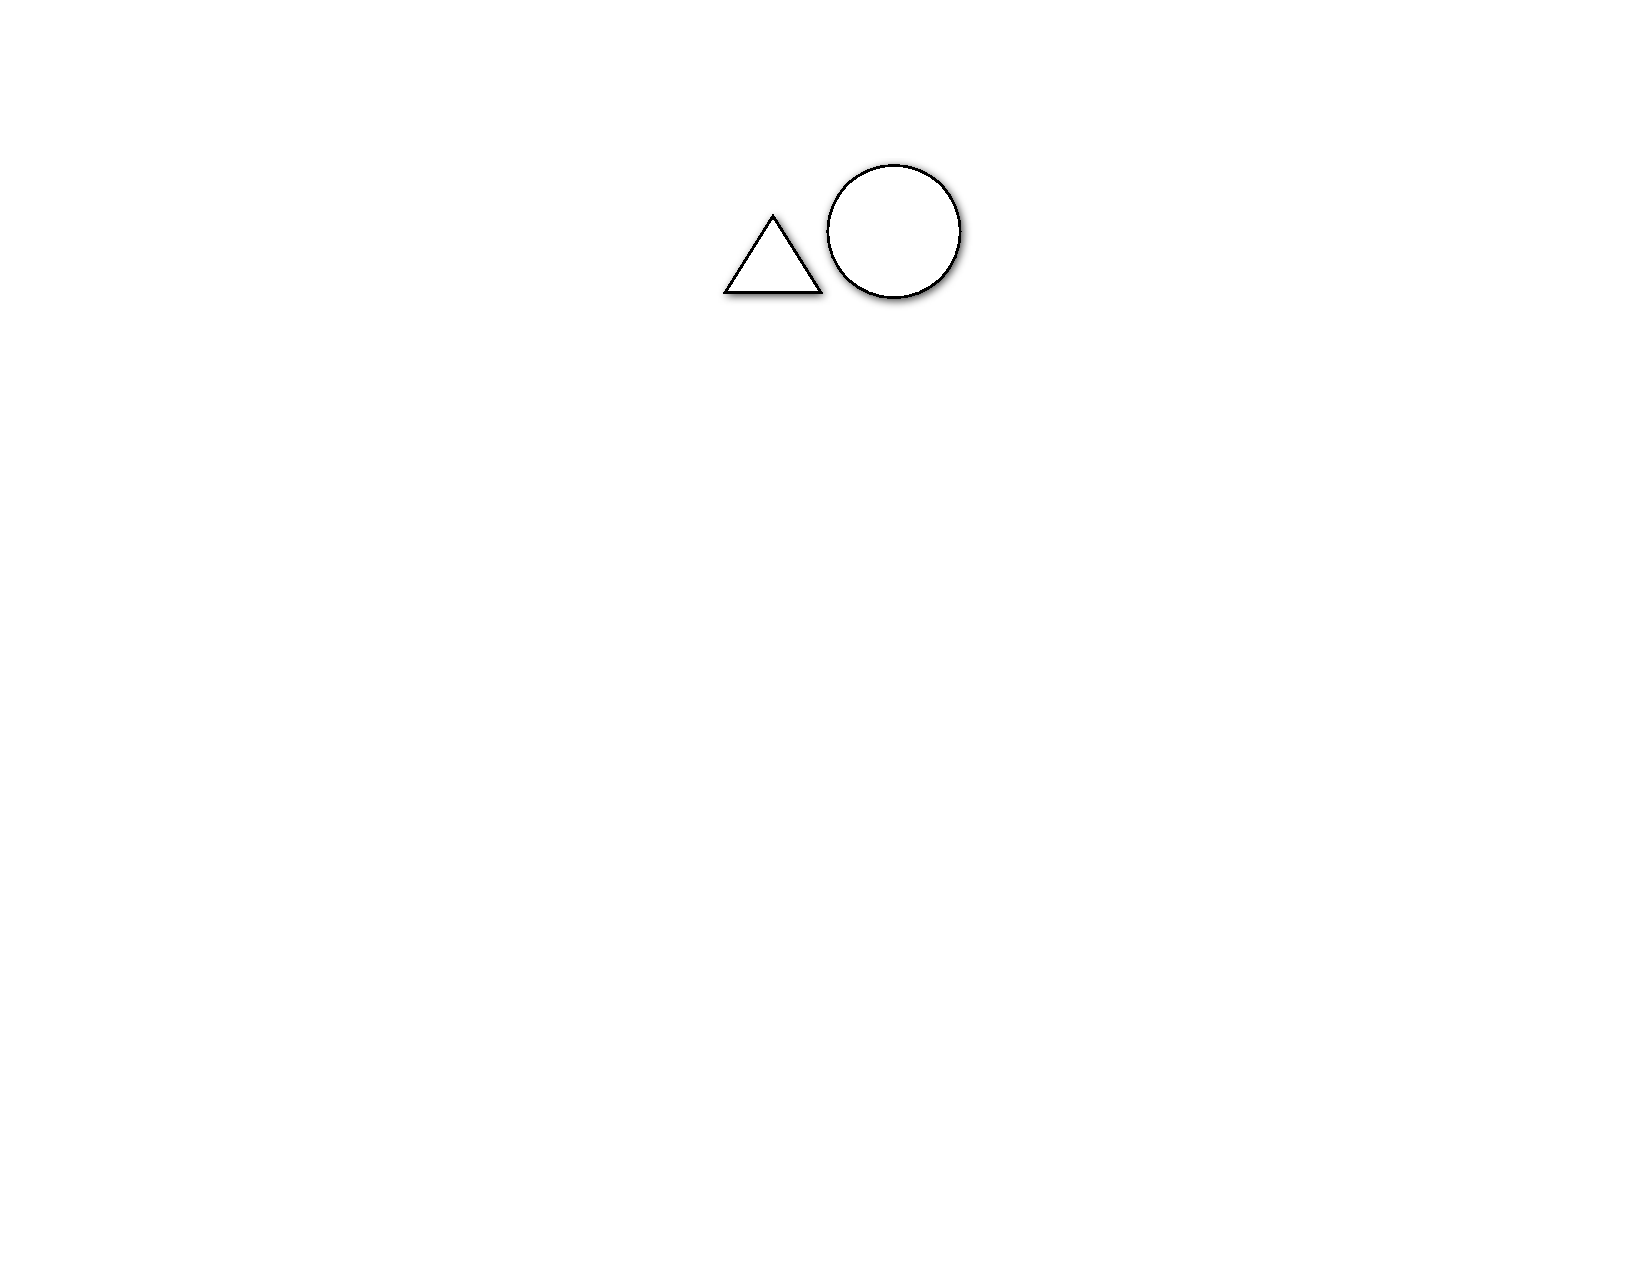
\includegraphics[width=0.4\textwidth]{triangle-circle}
% \end{center}
% \caption{A triangle and a circle.}
% \label{fig:triangle-circle}
% \end{figure}

\section{Deciding palindrome on a single tape TM}

The lower bound we are trying to prove is that there is a language \(L\) such that it can be decided within \(O(T(n))\)
time on a \(k\)-tape Turing Machine where \(k \geq 2\) but takes at least
\(O(T(n)^2)\) times on a single tape TM. We will 
exhibit this lower bound on \verb|PALINDROME|. We have seen that with \(2\)-tapes
we can solve \verb|PALINDROME| in \(O(n)\) time. So, the theorem we need to prove is as follows.

\begin{theorem}
    Deciding \verb|PALINDROME| requires \(\Omega(n^2)\) time on a single tape TM.
\end{theorem}

We have not yet discussed many sophisticated techniques for proving lower bounds. Still, this result is 
rather surprising and certainly non-trivial. Hence, proving it requires taking a fundamental approach.
In the process, we will find ourselves pondering over the very nature of information 
exchange. 

To aid this process, we will introduce some notiation. But first, it's important to develop some
intuition regarding why this result should be true. 

By restricting ourselves to one tape, we only have one \textit{source} of information i.e. the one head
that moves across the tape. We are asking the TM to verify that the string looks the same when read forwards or backwards.
Most importantly, we are asking it to do this without allowing it to \textit{copy} information from one place to 
another.\footnote[2]{At least to a place that can be conveniently accessed regularly, such as another tape.} As a result, 
any time the TM needs to make a comparison between two characters, the head needs to \textit{cross} over to the other side. 
In general, each crossing can take linear time and, since the comparison needs to be made about \(n/2\) times, the total 
runtime becomes quadratic. It seems as though asking for any better is unreasonable. But how can we know this for sure?

We recognized that the head needs to cross over to the second half of the word every time it makes
a comparison. So, one approach would be to show that in sub-quadratic time, there are simply not enough crossings that can be made to 
accurately distinguish all inputs \(x \in \left\{ 0,1 \right\}^n\). We now formalize this idea. 

\begin{definition}[crossing sequence]
    A crossing sequence \(C_i(x)\) is the sequence of states \((q_1, q_2. \ldots, q_k)\) of \(M\), run on input \(x\), where 
    \(q_k\) is the state of \(M\) immediately after crossing the \(i^{th}\) border of the tape (illustrated
    in Figure 3.4) for the \(k^{th}\) time.



\end{definition}

\begin{figure}[h]
\centering
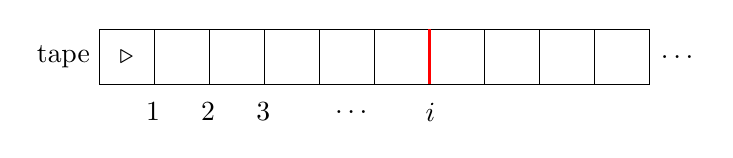
\begin{tikzpicture}
    


\edef\sizetape{0.7cm}
\tikzstyle{tmtape}=[draw,minimum size=\sizetape]
% \tikzstyle{tmhead}=[arrow box,draw,minimum size=.5cm,arrow box
% arrows={east:.25cm, west:0.25cm}]

%% Draw TM tape
\begin{scope}[shift={(-0.5cm,0cm)},start chain=1 going right,node distance=-0.15mm]
    \node [on chain=1,tmtape,draw=none] {tape};
    \node [on chain=1,tmtape] {\(\triangleright\)};
    \node [on chain=1,tmtape] (e) {};
    \node [on chain=1,tmtape] {};
    \node [on chain=1,tmtape] {};
    \node [on chain=1,tmtape] {};
    \node [on chain=1,tmtape] {};
    \node [on chain=1,tmtape] {};
    \node [on chain=1,tmtape] {};
    \node [on chain=1,tmtape] {};
    \node [on chain=1,tmtape] {};
    \node [on chain=1,tmtape,draw=none] {$\ldots$};
    % \node [on chain=1] {\textbf{Input/Output Tape}};

\end{scope}

    \node[text width = 1cm] at (1.05, -0.7) {1};
    \node[text width = 1cm] at (1.75, -0.7) {2};
    \node[text width = 1cm] at (2.45, -0.7) {3};
    \node[text width = 1cm] at (3.45, -0.7) {\ldots};
    \node[text width = 1cm] at (4.6, -0.7) {\(i\)};
    \draw[line width = 0.4mm, red] (4.15, 0.35) -- (4.15, -0.35);

\end{tikzpicture}
\caption{The \(i^{th}\) border of a tape}  
\end{figure}

\begin{remark}
    If the head of a TM never crosses \(i\) for a certain input \(x \in \left\{ 0,1 \right\}^n \) then \(C_i(x)\) is empty. 
    A crossing sequence is analagous to a customs officer that makes a certain observation about you (say the color of your t-shirt)
    and notes it down every time you cross the border.
\end{remark}

Next, we introduce and prove a lemma that provides the core of the theorem's proof.

\begin{lemma}
    Let \(M\) be a TM that decides some language \(L\). Let \(x,y\) be inputs 
    such that \(M(x) = M(y)\). Assume that we partition the input \(x\) at 
    some point \(i\) calling the left half \(x'\) and the right half \(x''\) 
    such that \(x = x'x''\). We do the same to \(y\) at \(j\) such that \(y = y'y''\).
    
    \begin{figure}[h]
        \centering
    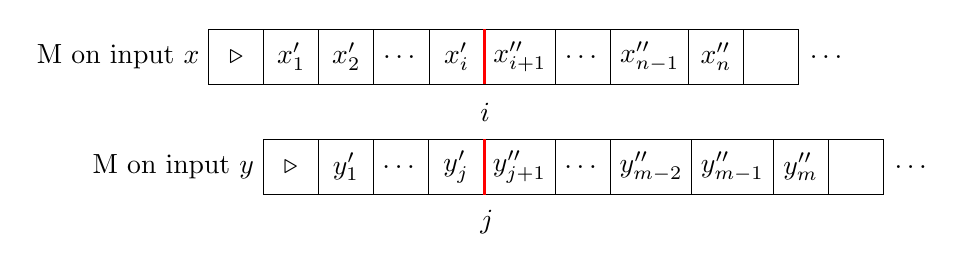
\begin{tikzpicture}
    


        \edef\sizetape{0.7cm}
        \tikzstyle{tmtape}=[draw,minimum size=\sizetape]
        % \tikzstyle{tmhead}=[arrow box,draw,minimum size=.5cm,arrow box
        % arrows={east:.25cm, west:0.25cm}]
        
        %% Draw TM tape
        \begin{scope}[shift={(-0.5cm,0cm)},start chain=1 going right,node distance=-0.15mm]
            \node [on chain=1,tmtape,draw=none] {M on input \(x\)};
            \node [on chain=1,tmtape] {\(\triangleright\)};
            \node [on chain=1,tmtape] {\(x_1'\)};
            \node [on chain=1,tmtape] {\(x_2'\)};
            \node [on chain=1,tmtape] {\ldots};
            \node [on chain=1,tmtape] {\(x_i'\)};
            \node [on chain=1,tmtape] {\(x_{i+1}''\)};
            \node [on chain=1,tmtape] {\ldots};
            \node [on chain=1,tmtape] {\(x_{n-1}''\)};
            \node [on chain=1,tmtape] {\(x_n''\)};
            \node [on chain=1,tmtape] {};
            \node [on chain=1,tmtape,draw=none] {$\ldots$};
            % \node [on chain=1] {\textbf{Input/Output Tape}};
        
        \end{scope}


        \begin{scope}[shift={(0.2cm,-1.4cm)},start chain=1 going right,node distance=-0.15mm]
            \node [on chain=1,tmtape,draw=none] {M on input \(y\)};
            % \node [on chain=1,tmtape] {\(\triangleright\)};
            \node [on chain=1,tmtape] {\(\triangleright\)};
            \node [on chain=1,tmtape] {\(y_1'\)};
            \node [on chain=1,tmtape] {\ldots};
            \node [on chain=1,tmtape] {\(y_j'\)};
            \node [on chain=1,tmtape] {\(y_{j+1}''\)};
            \node [on chain=1,tmtape] {\ldots};
            \node [on chain=1,tmtape] {\(y_{m-2}''\)};
            \node [on chain=1,tmtape] {\(y_{m-1}''\)};
            \node [on chain=1,tmtape] {\(y_m''\)};
            \node [on chain=1,tmtape] {};
            \node [on chain=1,tmtape,draw=none] {$\ldots$};
            % \node [on chain=1] {\textbf{Input/Output Tape}};
        
        \end{scope}
        
            % \node[text width = 1cm] at (1.05, -0.7) {1};
            % \node[text width = 1cm] at (1.75, -0.7) {2};
            % \node[text width = 1cm] at (2.45, -0.7) {3};
            % \node[text width = 1cm] at (3.45, -0.7) {\ldots};
            \node[text width = 1cm] at (4.6, -0.7) {\(i\)};
            \draw[line width = 0.4mm, red] (4.15, 0.35) -- (4.15, -0.35);

            \node[text width = 1cm] at (4.6, -2.1) {\(j\)};
            \draw[line width = 0.4mm, red] (4.15, -1.05) -- (4.15, -1.75);
        
    \end{tikzpicture}
    \caption{Partitioning \(x\) at \(i\) and \(y\) at \(j\)}
    \end{figure}

    Further, assume that \(C_i(x) = C_j(y)\). Then \(M(x'y'') = M(x) = M(y)\).
\end{lemma}

\begin{proof}
    The proof is best understood by visualizing running
    \(M\) on the hybrid input \(x'y''\). We will compare this to \(M\) running on \(x\) and \(y\) 
    illustrated in Figure 3.6.
    \begin{figure}[h]
    \centering
    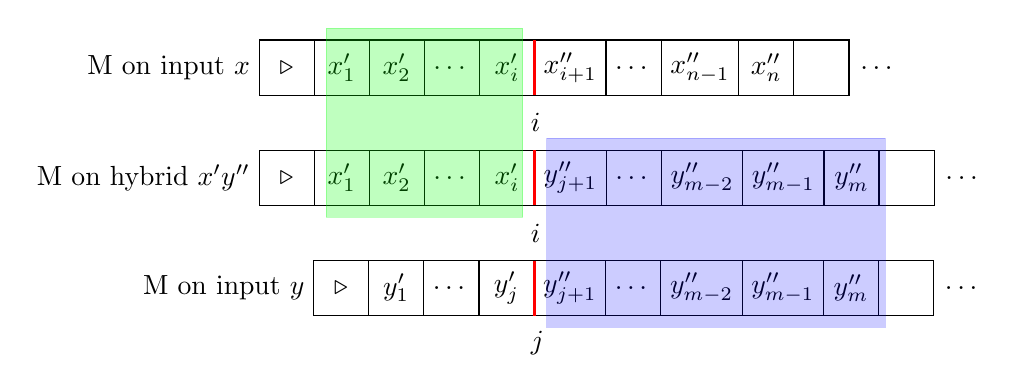
\begin{tikzpicture}
    


        \edef\sizetape{0.7cm}
        \tikzstyle{tmtape}=[draw,minimum size=\sizetape]
        % \tikzstyle{tmhead}=[arrow box,draw,minimum size=.5cm,arrow box
        % arrows={east:.25cm, west:0.25cm}]
        
        %% Draw TM tape
        \begin{scope}[shift={(-0.5cm,0cm)},start chain=1 going right,node distance=-0.15mm]
            \node [on chain=1,tmtape,draw=none] {M on input \(x\)};
            \node [on chain=1,tmtape] {\(\triangleright\)};
            \node [on chain=1,tmtape] {\(x_1'\)};
            \node [on chain=1,tmtape] {\(x_2'\)};
            \node [on chain=1,tmtape] {\ldots};
            \node [on chain=1,tmtape] {\(x_i'\)};
            \node [on chain=1,tmtape] {\(x_{i+1}''\)};
            \node [on chain=1,tmtape] {\ldots};
            \node [on chain=1,tmtape] {\(x_{n-1}''\)};
            \node [on chain=1,tmtape] {\(x_n''\)};
            \node [on chain=1,tmtape] {};
            \node [on chain=1,tmtape,draw=none] {$\ldots$};
            % \node [on chain=1] {\textbf{Input/Output Tape}};
        
        \end{scope}


        \begin{scope}[shift={(-0.82cm,-1.4cm)},start chain=1 going right,node distance=-0.15mm]
            \node [on chain=1,tmtape,draw=none] {M on hybrid \(x'y''\)};
            % \node [on chain=1,tmtape] {\(\triangleright\)};
            \node [on chain=1,tmtape] {\(\triangleright\)};
            \node [on chain=1,tmtape] {\(x_1'\)};
            \node [on chain=1,tmtape] {\(x_2'\)};
            \node [on chain=1,tmtape] {\ldots};
            \node [on chain=1,tmtape] {\(x_i'\)};
            \node [on chain=1,tmtape] {\(y_{j+1}''\)};
            \node [on chain=1,tmtape] {\ldots};
            \node [on chain=1,tmtape] {\(y_{m-2}''\)};
            \node [on chain=1,tmtape] {\(y_{m-1}''\)};
            \node [on chain=1,tmtape] {\(y_m''\)};
            \node [on chain=1,tmtape] {};
            \node [on chain=1,tmtape,draw=none] {$\ldots$};
            % \node [on chain=1] {\textbf{Input/Output Tape}};
        
        \end{scope}

        \begin{scope}[shift={(0.2cm,-2.8cm)},start chain=1 going right,node distance=-0.15mm]
            \node [on chain=1,tmtape,draw=none] {M on input \(y\)};
            % \node [on chain=1,tmtape] {\(\triangleright\)};
            \node [on chain=1,tmtape] {\(\triangleright\)};
            \node [on chain=1,tmtape] {\(y_1'\)};
            \node [on chain=1,tmtape] {\ldots};
            \node [on chain=1,tmtape] {\(y_j'\)};
            \node [on chain=1,tmtape] {\(y_{j+1}''\)};
            \node [on chain=1,tmtape] {\ldots};
            \node [on chain=1,tmtape] {\(y_{m-2}''\)};
            \node [on chain=1,tmtape] {\(y_{m-1}''\)};
            \node [on chain=1,tmtape] {\(y_m''\)};
            \node [on chain=1,tmtape] {};
            \node [on chain=1,tmtape,draw=none] {$\ldots$};
            % \node [on chain=1] {\textbf{Input/Output Tape}};
        
        \end{scope}
        
            % \node[text width = 1cm] at (1.05, -0.7) {1};
            % \node[text width = 1cm] at (1.75, -0.7) {2};
            % \node[text width = 1cm] at (2.45, -0.7) {3};
            % \node[text width = 1cm] at (3.45, -0.7) {\ldots};
            \node[text width = 1cm] at (4.6, -0.7) {\(i\)};
            \draw[line width = 0.4mm, red] (4.15, 0.35) -- (4.15, -0.35);

            \node[text width = 1cm] at (4.6, -2.1) {\(i\)};
            \draw[line width = 0.4mm, red] (4.15, -1.05) -- (4.15, -1.75);

            \node[text width = 1cm] at (4.6, -3.5) {\(j\)};
            \draw[line width = 0.4mm, red] (4.15, -2.45) -- (4.15, -3.15);

            \draw[green, fill = green, opacity = 0.25] (1.5,0.5) rectangle (4,-1.9);
            \draw[blue, fill = blue, opacity = 0.2] (4.3,-0.9) rectangle (8.6,-3.3);
        
    \end{tikzpicture}
    \caption{Comparing \(M\) on hybrid input with \(M\) on \(x\) and \(y\)}
    \end{figure}
    Let's simulate \(M\) on \(x'y''\). Clearly, until the \(i^{th}\) border is crossed for the first time
    \(M(x'y'')\) runs in the exact same way as \(M(x)\). Once \(i\) is crossed, \(M(x'y'')\) runs like \(M(y)\) until \(i\) is crossed again. In this way, 
    we can partition the computation period on \(x'y''\) into multiple intervals, each separated by a crossing of \(i\). These intervals can be classified
    into two types: one, colored in green, where the head stays to the left of \(i\) and one, colored in blue, where the head stays to the right of \(i\). Each left (right) interval corresponds to some
    sequence of computations on \(x \; (y)\) where the head stays in \(x' \; (y'')\).

    Further, we are given that \(C_i(x) = C_j(y)\). This means that \(\forall k \in \left\{1,2,\ldots, |C_i(x)| \right\}\) the state of \(M\) running on \(x\) when the head crosses the \(i^{th}\) border for the \(k^{th}\) time is the same
    as the state of \(M\) running on \(y\) when the head crosses the \(j^{th}\) border for the \(k^{th}\) time. Matthew summarizes this by observing that when \(M\) runs on \(x'y''\), it thinks that it is running on either \(x\) 
    or \(y\) (depending on the computational interval) and preserves its state when crossing the border between the two. As a result, \(M\) decides on the hybrid input the same way it decides on \(x\) and \(y\).
\end{proof}

Now we will prove the theorem. Informally, will we show that for a certain class of inputs, there must be many distinct crossing sequences. 
As a result, there must be some input \(x\) of this type that has long (in the order of \(O(n)\)) crossing sequences at \(n\) different borders. Therefore, 
the \(TM\) must take at least \(O(n^2)\) time to compute it.

\begin{proof}[Proof of theorem]
    We have shown that if \(M\) 
    decides the same for two inputs \(x\) and \(y\) and they have the same crossing sequences 
    \(C_i(x)\) and \(C_j(y)\) for any \(i \in \left\{ 1,2, \ldots, |x| \right\},j \in \left\{ 1,2,\ldots, |y| \right\}\), 
    then we can create a hybrid input \(x'y''\) for which \(M(x'y'') = M(x) = M(y)\). 
    
    We use the contrapositive of this lemma by fixing two inputs of the form \(x0^nx^R\) and \(y0^ny^R\) where \(x\neq y\). 
    Here \(x^R\) denotes \(x\) reversed i.e. read from right to left. \\

    \begin{figure}[h]
    \centering
    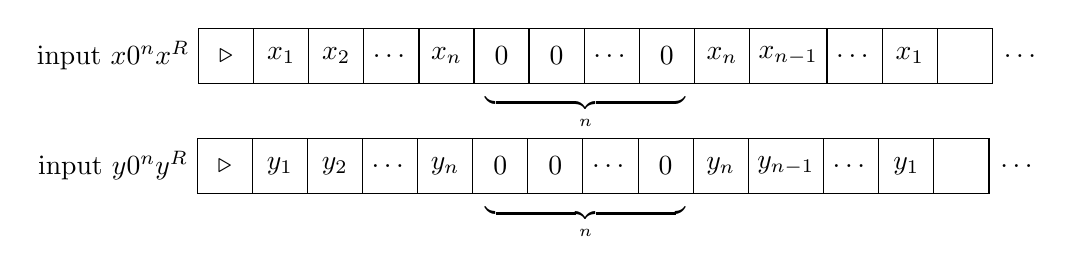
\begin{tikzpicture}
    


        \edef\sizetape{0.7cm}
        \tikzstyle{tmtape}=[draw,minimum size=\sizetape]
        % \tikzstyle{tmhead}=[arrow box,draw,minimum size=.5cm,arrow box
        % arrows={east:.25cm, west:0.25cm}]
        
        %% Draw TM tape
        \begin{scope}[shift={(-0.5cm,0cm)},start chain=1 going right,node distance=-0.15mm]
            \node [on chain=1,tmtape,draw=none] {input \(x0^nx^R\)};
            \node [on chain=1,tmtape] {\(\triangleright\)};
            \node [on chain=1,tmtape] {\(x_1\)};
            \node [on chain=1,tmtape] {\(x_2\)};
            \node [on chain=1,tmtape] {\ldots};
            \node [on chain=1,tmtape] {\(x_n\)};
            \node [on chain=1,tmtape] {\(0\)};
            \node [on chain=1,tmtape] {\(0\)};
            \node [on chain=1,tmtape] {\ldots};
            \node [on chain=1,tmtape] {\(0\)};
            \node [on chain=1,tmtape] {\(x_n\)};
            \node [on chain=1,tmtape] {\(x_{n-1}\)};
            \node [on chain=1,tmtape] {\ldots};
            \node [on chain=1,tmtape] {\(x_1\)};
            \node [on chain=1,tmtape] {};
            \node [on chain=1,tmtape,draw=none] {$\ldots$};
            % \node [on chain=1] {\textbf{Input/Output Tape}};
        
        \end{scope}

        \begin{scope}[shift={(-0.5cm,-1.4cm)},start chain=1 going right,node distance=-0.15mm]
            \node [on chain=1,tmtape,draw=none] {input \(y0^ny^R\)};
            \node [on chain=1,tmtape] {\(\triangleright\)};
            \node [on chain=1,tmtape] {\(y_1\)};
            \node [on chain=1,tmtape] {\(y_2\)};
            \node [on chain=1,tmtape] {\ldots};
            \node [on chain=1,tmtape] {\(y_n\)};
            \node [on chain=1,tmtape] {\(0\)};
            \node [on chain=1,tmtape] {\(0\)};
            \node [on chain=1,tmtape] {\ldots};
            \node [on chain=1,tmtape] {\(0\)};
            \node [on chain=1,tmtape] {\(y_n\)};
            \node [on chain=1,tmtape] {\(y_{n-1}\)};
            \node [on chain=1,tmtape] {\ldots};
            \node [on chain=1,tmtape] {\(y_1\)};
            \node [on chain=1,tmtape] {};
            \node [on chain=1,tmtape,draw=none] {$\ldots$};
            % \node [on chain=1] {\textbf{Input/Output Tape}};
        
        \end{scope}

        
        
            % \node[text width = 1cm] at (1.05, -0.7) {1};
            % \node[text width = 1cm] at (1.75, -0.7) {2};
            % \node[text width = 1cm] at (2.45, -0.7) {3};
            % \node[text width = 1cm] at (3.45, -0.7) {\ldots};
            \node[] at (5.5, -0.7) {\footnotesize \(\underbrace{\hphantom{00000000000000000}}_{n}\)};
            \node[] at (5.5, -2.1) {\footnotesize \(\underbrace{\hphantom{00000000000000000}}_{n}\)};
            % \draw[line width = 0.4mm, red] (4.15, 0.35) -- (4.15, -0.35);
        
    \end{tikzpicture}
    \caption{Constructing inputs that are forced to be palidromes}
    \end{figure}

    Clearly, both are palindromes so \(M(x) = M(y) = 1\)
    but for any \(i, j \in \left\{ n+1, n+2, \ldots, 2n \right\}\) we have \(C_i(x0^nx^R) \neq C_j(y0^ny^R)\) since the hybrids corresponding 
    to these indices cannot be palidromes (by the assumption \(x \neq y\)). \\

    \begin{figure}[h]
    \centering
    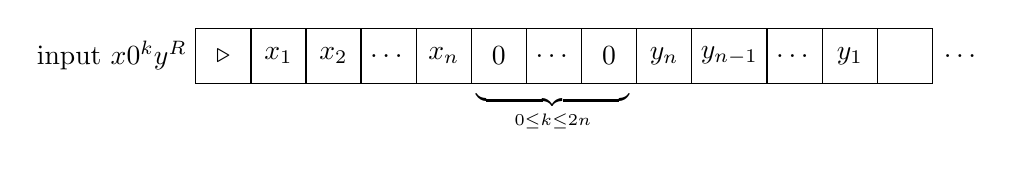
\begin{tikzpicture}
    


        \edef\sizetape{0.7cm}
        \tikzstyle{tmtape}=[draw,minimum size=\sizetape]
        % \tikzstyle{tmhead}=[arrow box,draw,minimum size=.5cm,arrow box
        % arrows={east:.25cm, west:0.25cm}]
        
        %% Draw TM tape
        \begin{scope}[shift={(-0.5cm,0cm)},start chain=1 going right,node distance=-0.15mm]
            \node [on chain=1,tmtape,draw=none] {input \(x0^ky^R\)};
            \node [on chain=1,tmtape] {\(\triangleright\)};
            \node [on chain=1,tmtape] {\(x_1\)};
            \node [on chain=1,tmtape] {\(x_2\)};
            \node [on chain=1,tmtape] {\ldots};
            \node [on chain=1,tmtape] {\(x_n\)};
            \node [on chain=1,tmtape] {\(0\)};
            \node [on chain=1,tmtape] {\ldots};
            \node [on chain=1,tmtape] {\(0\)};
            \node [on chain=1,tmtape] {\(y_n\)};
            \node [on chain=1,tmtape] {\(y_{n-1}\)};
            \node [on chain=1,tmtape] {\ldots};
            \node [on chain=1,tmtape] {\(y_1\)};
            \node [on chain=1,tmtape] {};
            \node [on chain=1,tmtape,draw=none] {$\ldots$};
            % \node [on chain=1] {\textbf{Input/Output Tape}};
        
        \end{scope}

        
        
        % \node[text width = 1cm] at (1.05, -0.7) {1};
        % \node[text width = 1cm] at (1.75, -0.7) {2};
        % \node[text width = 1cm] at (2.45, -0.7) {3};
        % \node[text width = 1cm] at (3.45, -0.7) {\ldots};
        \node[] at (5.1, -0.7) {\footnotesize \(\underbrace{\hphantom{0000000000000}}_{0 \leq k \leq 2n}\)};
        % \draw[line width = 0.4mm, red] (4.15, 0.35) -- (4.15, -0.35);
    
    \end{tikzpicture}
    \caption{Example of \(2n\) different hybrids that are not palidromes}
    \end{figure}
    
    Therefore, if we restrict ourselves to inputs of the form \(x0^nx^R, x \in \left\{ 0,1 \right\}^n\) we observe that for for all indices \(i \in \left\{ n+1, n+2, \ldots, 2n \right\}\), 
    as we range over all possible \(x \in \left\{ 0,1 \right\}^n\), the crossing sequences \(C_i(x0^nx^R)\) must be distinct. 

    \begin{remark}
            The previous sentence had multiple quantifiers so it is worth re-reading it
            to appreciate just how many distinct crossing sequences we have found. For each \(i\), we have found \(2^n\) distinct crossing sequences, each corresponding to some \(x \in \left\{ 0,1 \right\}^n\).
    \end{remark}

    To accomodate all these distinct crossing sequences, we inevitably need some sequences that are long. Specifically, if the longest sequence has length \(l\) and the number of states that the TM can represent
    is \(|Q|\), then the total number of distinct crossing sequences is \(\sum\limits_{k=1}^{l}|Q|^k \leq (|Q| + 1)^l\) which is relatively small in size unless \(l\) is large. So for each \(i\), if we have to accomodate
    \(2^n\) distinct sequences, then by the pigeonhole principle we need at least one sequence with large length \(l\) where \((|Q| + 1)^l \geq 2^n \). Writing this with quantifiers and rearranging terms
    \begin{equation}
        \forall i \in \left\{ n+1, n+2, \ldots, 2n\right\}\; \exists x \in \left\{ 0,1 \right\}^n : |C_i(x0^nx^R)| \geq \dfrac{n}{\log(|Q| + 1)} = \Omega(n)
    \end{equation}
    
    We now simply switch the order of the quantifiers. 
    
    \begin{equation}
        \exists x \in \left\{ 0,1 \right\}^n \; \forall i \in \left\{ n+1, n+2, \ldots, 2n\right\} : |C_i(x0^nx^R)| \geq \dfrac{n}{\log(|Q| + 1)} = \Omega(n)
    \end{equation}
    
    In words, there is some input \(x0^nx^R\) such that for \(n\) different indices \(i\), the \(i^{th}\) border is crossed at least \(n\) times. 
    In total, there are \(n\) different borders each of which is crossed at least \(n\) times. So, \(M\) takes at least \(n^2\) steps to halt on the input \(x0^nx^R\). 
    This concludes our proof that the running time of \(M\) is \(\Omega(n^2)\).
\end{proof}

\begin{remark}
    The hybrid approach used in this proof is common
    in theoretical computer science. It is used when
    there are two interesting features exhibited in 
    two different cases. We then try to construct a 
    hybrid scenario where both phenomena can be seen together.
    Matan adds that this approach is commonly used in proving
    lower bounds in cryptography. 
\end{remark}

\begin{problem}
    Prove that computing \(f: x \mapsto xx\) requires \(\Omega(n^2)\) time on a single tape TM. 
\end{problem}

\begin{problem}
    We are given a turing machine \(M\) that decides some language \(L\) in \(O(n)\). What speed-up can be achieved with a \(k\)-tape machine?
\end{problem}

\begin{problem}
    Prove that if \(f: \left\{ 0,1 \right\}^* \to \left\{ 0,1 \right\}^*\) is computable in time \(T(n)\) with \(k\) tapes, then it can computed in time \(O(T(n)\log T(n))\) using \(2\) tapes. 
\end{problem}

\begin{remark}
    In fact, a logarithmic slowdown is so insigniciant that we use the notation \(\tilde{O}(T(n)) = O(T(n)\log T(n))\).
\end{remark}

\begin{problem}
    From the Problem 3.20, a \(k\)-tape TM can be replaced with a \(2\)-tape TM without a significant slowdown. What additional \textit{functionality} do we get by using two tapes over one?
\end{problem}

% \section{Mathematical environments}


% \noindent
% Note that \LaTeX\ automatically numbers these
% environments within the lecture number (\thelecture\ in
% this case).  The same applies to the numbering of pages
% (this page being page \thepage), figures
% (Figure~\ref{fig:triangle-circle} above), and
% equations:
% \begin{align}
% a = a_1+a_2+\cdots+a_n.
% \end{align}
% \noindent
% For proofs, use the provided {\tt proof} environment,
% illustrated below.


\bibliographystyle{abbrv}
\bibliography{template}

\end{document}
